\chapter{Практическое применение модели}
Понимание того, как будет работать модель на практике, важная часть исследовательской деятельности. На основе экспериментов можно будет давать практические рекомендации по подбору параметров, спецификации при использовании. Правильная постановка эксперимента позволит сравнить предложенный метод с бейзлайном.

\section{Описание данных}
\note{Этап создания алгоритмов}
Инфраструктура, созданная в компании предусматривает взаимодействие с широким кругом лиц, которые внештатно создают торговые стратегии, получая за это небольшое вознаграждение. При написании алгоритма можно:
\begin{enumerate}
	\item выбрать торгуемые активы
	\item задать периодичность, с которой работает алгоритм
	\item собирать любые статистики с предыдущих периодов
	\item произвольным образом реструктурировать портфель основываясь на прошлой информации
\end{enumerate}
Обладая навыками программирования на \texttt{Python}, можно написать любую стратегию, которая использует только рыночные данные. Алгоритмов огромное количество, более 700 000, большинство из этих алгоритмов написаны энтузиастами. В отличие от рыночных активов, которых ограниченное количество, алгоримов гораздо больше. Это открывает широкие возможности для применения портфельной теории для создания диверсифицированного портфеля.

\note{Этап селекции алгоритмов}
Тем не менее, применять портфельную теорию проблематично. Для такого количества временных рядов длина ряда слишком мала. Расчет даже ковариационной матрицы требует огромных вычислительных мощностей и памяти. Для решения этой проблемы существует этап предварительного отбора алгоритмов, этап селекции. В инфраструктуре разработана модель, которая выбирает наиболее стабильные из совокупности\footnote{Детали реализации защищены NDA}. После этого этапа остается около 150 торговых стратегий, которые и были использованы для тестирования модели динамики торговых стратегий.

\section{Выбор спецификации модели}
\note{Эмпирический анализ корреляционных матриц}
\begin{figure}[t]
	\centering
	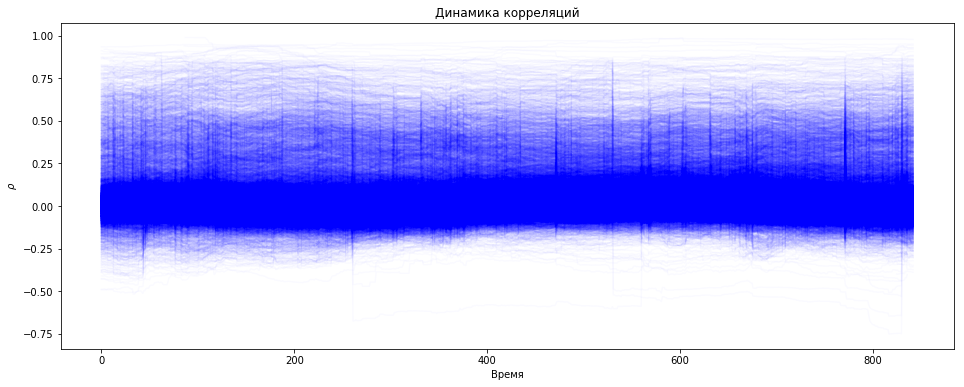
\includegraphics[width=\linewidth]{Thesis/images/correlations}
	\caption{График динамики корреляций между торговыми стратегиями. Попарные корреляции были посчитаны за период 2013-2017 с окном 300 дней. Не наблюдается существенного изменения корреляций за этот период.}
	\label{fig:correlations}
\end{figure}
Этап селекции имел важные последствия на спецификацию модели. Отобранные алгоритмы имели существенно другие распределения статистик. Предположение о динамики корреляций оказалось не состоятельным (Рисунок \ref{fig:correlations}). В данных не наблюдается существенного изменения корреляций для большой группы торговых стратегий. Выводы, которые можно сделать на основе этого графика:
\begin{enumerate}
	\item корреляции относительно стабильны во времени
	\item большинство корреляций околонулевые
\end{enumerate}

Основываясь на этих выводах остается сфокусироваться на двух спецификациях, которые не учитывают динамику корреляций:
\begin{itemize}
	\item модель без корреляций \eqref{eq:nocorr}
	\item модель со статичными корреляциями \eqref{eq:staticcorr}
\end{itemize}

\section{Постановка эксперимента и оценка модели}
\note{Описание поставленного эксперимента}
Для качественных выводов о работе предложенного метода составления портфеля недостаточно оценить одну модель на подвыборке алгоритмов, так как это может быть случайный успех или неудача. Для проведения эксперимента на реальных данных был использован метод бутстрэп \citep{grimshaw1995} и разделение выборки на обучающую и тестовую. 

\begin{itemize}
	\item Всего 4 года наблюдений
	\item Обучающая выборка -- первые два года
	\item Тестовая выборка -- последние два года
	\item Сгенерировано 400 выборок алгоритмов размера 20 из 150 без повторений
	\item Двумя методами: предложенным и по Марковицу, строятся портфели основываясь на данных обучающей выборки
	\item Считается критерий качества (коэффициент Шарпа) на тестовой выборке
\end{itemize}

\note{Параметры NUTS}
Для оценки апостериорных распределений параметров модели использовался зарекомендовавший себя алгоритм NUTS \citep{hoffman2011nuts}, при этом генерировалась выборка размера 3000 из этого распределения. Для оценки потребовались большие вычислительные мощности. Так, расчет модели на динамику 20-ти алгоритмов со статическими корреляциями \eqref{eq:staticcorr} занимает около 3х часов на 32х-ядерном сервере. Оценка модели без корреляций \eqref{eq:nocorr} занимает около получаса. 

\section{Сравнение метода с портфельной теорией Марковица}
\begin{figure}[t]
	\centering
	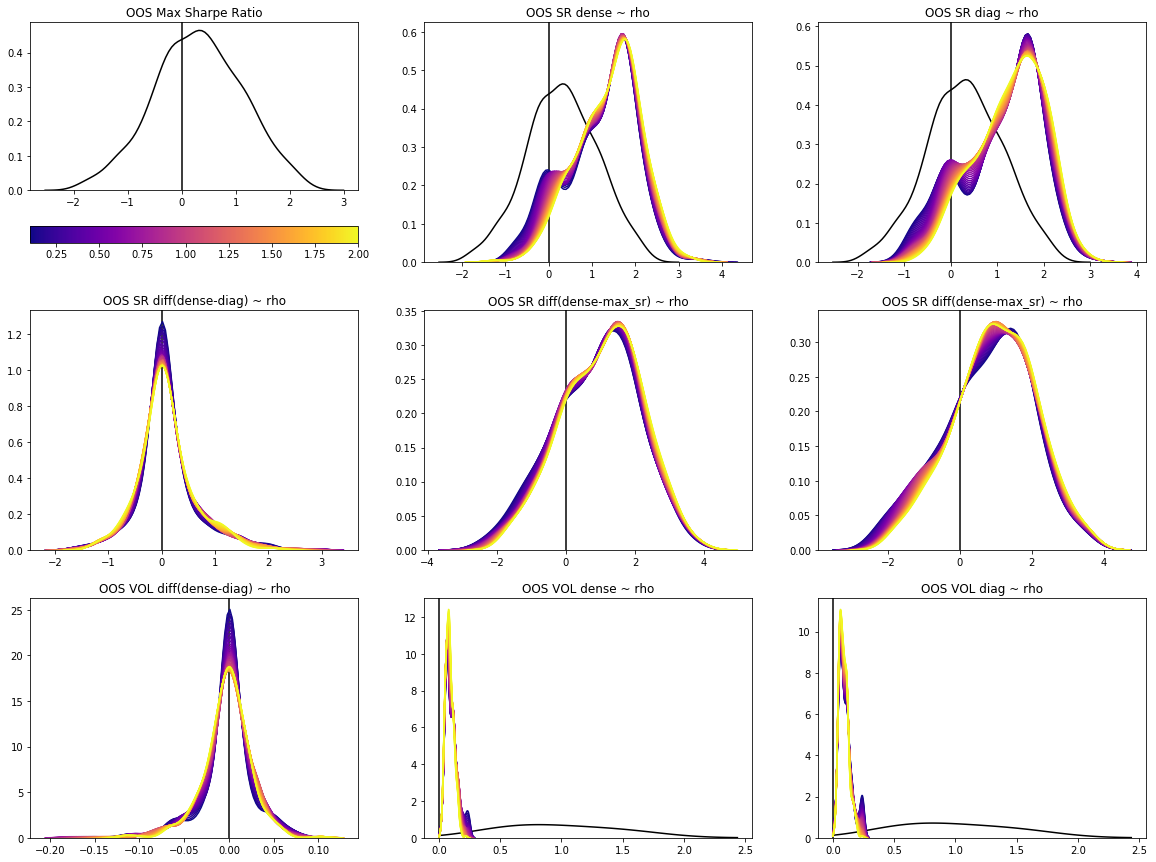
\includegraphics[width=\linewidth]{Thesis/images/performance}
	\caption{Сравнение коэффициента Шарпа на тестовой выборке байесовского (выделен цветом) и оптимального портфеля Марковица. Цветовая шкала означает значение параметра $\rho$ в функции полезности \eqref{eq:isoelastic}. Распределение коэффициента Шарпа на тестовом периоде находится значительно правее, что означает преимущество предложенного метода над ранее используемым аналогом}
	\label{fig:performance}
\end{figure}

\note{Описание и трактовка результатов}

Из экспериментов следует, что предложенный алгоритм более устойчив при обучении, обладает необходимой обобщающей способностью для улучшения качества портфеля по ряду показателей. В целом не важно, какую спецификацию модели выбирать: дополнительное моделирование корреляций не принесло большой пользы, разница волатильности и коэффициентов Шарпа между моделью \eqref{eq:staticcorr} и \eqref{eq:nocorr} имеет сконцентрированное в нуле распределение.

\begin{itemize}
	\item Коэффициент Шарпа: в 70\% случайно выбранных портфелях коэффициент Шарпа больше полученного методом Марковица
	\item Дисперсия получаемого портфеля новым способом ниже
	\item Моделирование корреляций не дает существенного преимущества перед моделью без них
\end{itemize}

